\documentclass{article}

\usepackage{fancyhdr}
\usepackage{extramarks}
\usepackage{amsmath}
\usepackage{amsthm}
\usepackage{amsfonts}
\usepackage{tikz}
\usepackage[plain]{algorithm}
%\usepackage{algpseudocode}
\usepackage{amssymb}
\usepackage{enumitem}
\usepackage{relsize}
\usepackage{textcomp}
\usepackage{graphicx}
\usepackage{bm}
\usepackage{wasysym}
%\usepackage{textcomp}
%\usepackage{tabularx}
\usepackage{xcolor,colortbl}

%\usetikzlibrary{automata,positioning}
%\usepgfplotslibrary{external} 
%\tikzexternalize

%
% Basic Document Settings
%

\topmargin=-0.45in
\evensidemargin=0in
\oddsidemargin=0in
\textwidth=6.5in
\textheight=9.0in
\headsep=0.25in

\linespread{1.1}

\pagestyle{fancy}
\lhead{\hmwkAuthorName}
\chead{\hmwkClass\ (\hmwkClassInstructor\ \hmwkClassTime): \hmwkTitle}
\rhead{\hmwkDueDate}
\lfoot{\lastxmark}
\cfoot{\thepage}

\newcommand{\minus}{\scalebox{0.5}[1.0]{$-$}}
\newcommand\tab[1][0.5cm]{\hspace*{#1}}
\renewcommand\headrulewidth{0.4pt}
\renewcommand\footrulewidth{0.4pt}
\renewcommand{\theenumi}{\Alph{enumi}}

\setlength\parindent{0pt}

%
% Create Problem Sections
%

\newcommand{\enterProblemHeader}[1]{
	\nobreak\extramarks{}{{#1} continued on next page\ldots}\nobreak{}
	\nobreak\extramarks{{#1} (continued)}{{#1} continued on next page\ldots}\nobreak{}
}

\newcommand{\exitProblemHeader}[1]{
	\nobreak\extramarks{{#1} (continued)}{{#1} continued on next page\ldots}\nobreak{}
	\stepcounter{homeworkProblemCounter}
	\nobreak\extramarks{{#1}}{}\nobreak{}
}

\newcounter{homeworkProblemCounter}
\setcounter{secnumdepth}{0}
\newcounter{partCounter}
\nobreak\extramarks{Problem \arabic{homeworkProblemCounter}}{}\nobreak{}

\newenvironment{homeworkProblem}[1][-1]{
	\subsection*{{#1}:}
	\enterProblemHeader{{#1}}
	\exitProblemHeader{{#1}}
}

\newcommand{\hmwkTitle}{Homework 5}
\newcommand{\hmwkDueDate}{November 18, 2019}
\newcommand{\hmwkClass}{MTH 5051}
\newcommand{\hmwkClassTime}{Section 01}
\newcommand{\hmwkClassInstructor}{Dr. Jim Jones}
\newcommand{\hmwkAuthorName}{\textbf{Eric Pereira}}

%
% Title Page
%
\pagenumbering{gobble}
\title{
	\vspace{2in}
	\textmd{\textbf{\hmwkClass:\ \hmwkTitle}}\\
	\normalsize\vspace{0.1in}\small{Due\ on\ \hmwkDueDate\ at 11:59pm}\\
	\vspace{0.1in}\large{\textit{\hmwkClassInstructor\ \hmwkClassTime}}
	\vspace{3in}
}

\author{\hmwkAuthorName}
\date{}

\renewcommand{\part}[1]{\textbf{\large Part \Alph{partCounter}}\stepcounter{partCounter}\\}

%
% Various Helper Commands
%

% Useful for algorithms
\newcommand{\alg}[1]{\textsc{\bfseries \footnotesize #1}}

% For derivatives
\newcommand{\deriv}[1]{\frac{\mathrm{d}}{\mathrm{d}x} (#1)}

% For partial derivatives
\newcommand{\pderiv}[2]{\frac{\partial}{\partial #1} (#2)}

% Integral dx
\newcommand{\dx}{\mathrm{d}x}

% Alias for the Solution section header
\newcommand{\solution}{\textbf{\large Solution}}

% Probability commands: Expectation, Variance, Covariance, Bias
\newcommand{\E}{\mathrm{E}}
\newcommand{\Var}{\mathrm{Var}}
\newcommand{\Cov}{\mathrm{Cov}}
\newcommand{\Bias}{\mathrm{Bias}}

\begin{document}
	\maketitle
	
	\pagebreak
	\pagenumbering{arabic}
	
	
	%%%%%%%%%%%%%%%%%%%      
	%	NEW SECTION   %
	%%%%%%%%%%%%%%%%%%%
	\section{Chapter 11.1}
	
	%%%%%%%%%%%%%%%%%%%%%%%%%%%%%%%%%%%%%%%%%%%%%%%%%%%%%%%%%%%%%%%%%%%%%%%%%%%%%%%%%%
	%                                                                                %
	%                          Section 11.1 Problem 2                                %
	%                                                                                %
	%%%%%%%%%%%%%%%%%%%%%%%%%%%%%%%%%%%%%%%%%%%%%%%%%%%%%%%%%%%%%%%%%%%%%%%%%%%%%%%%%%
	
	\begin{homeworkProblem}[Problem 2]
		\tab For the graph in Fig. 11.7, determine 
		\begin{enumerate}[label=\alph*)]
			\item a walk from $b$ to $d$ that is not a trail;
			\item a $b$-$d$ trail that is not a path;
			\item a path from $b$ to $d$;
			\item a closed walk from $b$ to $b$ that is not a circuit;
			\item a circuit from $b$ to $b$ that is not a cycle; and
			\item a cycle from $b$ to $b$.
		\end{enumerate}
		
		\begin{center}
			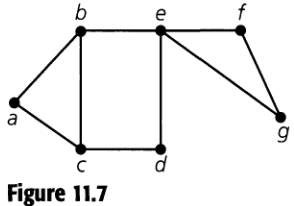
\includegraphics[scale=.7]{photos/117.png}
		\end{center}
		
		\textbf{\\Solution:}
		\begin{enumerate}[label=\alph*)]
			\item A trail would be from points $b$ to $d$ where no edge is repeated. In this case all we would have to do is repeat an edge. To do this we could write:
				\begin{align*}
					\bm{\{b,e\}, \{e,b\}, \{b,e\}, \{e,d\}}
				\end{align*}
			\item A path is much like a trail, except no vertex is repeated twice. As a result the same answer from the last question can be used to answer this:
				\begin{align*}
					\bm{\{b,e\}, \{e,b\}, \{b,e\}, \{e,d\}}
				\end{align*}
			\item A path from $b$ to $d$ would look like:
				\begin{align*}
					\bm{\{b,e\}, \{e,d\}}
				\end{align*}
			\item A circuit is a closed x-x trail, meaning x eventually ends up at itself again. So, in order to do this we just have to make sure it is not a trail. This could look like:
				\begin{align*}
					\bm{\{b,e\}, \{e,b\}}
				\end{align*}
			\item A cycle is a closed x-x path, so we have to create an x-x trail that is also not a path. This would look like:
				\begin{align*}
					\bm{\{b,e\}, \{e,f\}, \{f,g\}, \{g,e\}, \{e,d\}, \{d,c\}, \{c,b\}}
				\end{align*}
			\item An easy cycle, that also happens to be a circuit, is:
				\begin{align*}
					\bm{\{b,a\}, \{a,c\}, \{c,b\}}
				\end{align*}
		\end{enumerate}
		
	\end{homeworkProblem} 


	%%%%%%%%%%%%%%%%%%%%%%%%%%%%%%%%%%%%%%%%%%%%%%%%%%%%%%%%%%%%%%%%%%%%%%%%%%%%%%%%%%
	%                                                                                %
	%                          Section 11.1 Problem 7                                %
	%                                                                                %
	%%%%%%%%%%%%%%%%%%%%%%%%%%%%%%%%%%%%%%%%%%%%%%%%%%%%%%%%%%%%%%%%%%%%%%%%%%%%%%%%%%
	
	\begin{homeworkProblem}[Problem 7]
		\tab Seven towns $a$, $b$, $c$, $d$, $e$, $f$, and $g$ are connected by a system of highways as follows:
		
		\begin{center}
			\begin{enumerate}[label=(\arabic*)]
				\item I-22 goes from $a$ to $c$ passing through $b$;
				\item 1-33 goes from $c$ to $d$ and then passes through $b$ as it continues to $f$;
				\item 1-44 goes from $d$ through $e$ to $a$;
				\item 1-55 goes from $f$ to $b$, passing through $g$; and
				\item 1-66 goes from $g$ to $d$.
			\end{enumerate}
		\end{center}
	
		 \bigskip
	
		\begin{enumerate}[label=(\alph*)]
			\item Using vertices for towns and directed edges for segments of highways between towns, draw a directed graph that models this situation.
			\item List the paths from $g$ to $a$.
			\item What is the smallest number of highway segments that would have to be closed down in order for travel from $b$ to $d$ to be disrupted?
			\item Is it possible to leave town $c$ and return there, visiting each of the other towns only once?
			\item What is the answer to part (d) if we are not required to return to $c$?
			\item Is it possible to start at some town and drive over each of these highways exactly once? (You are allowed to visit a town more than once, and you need not return to the town from which you started.)
		\end{enumerate}
		\textbf{\\Solution:}
		
		\begin{enumerate}[label=(\alph*)]
			\item Here is a self made representation of the map: \\
				\begin{center}
					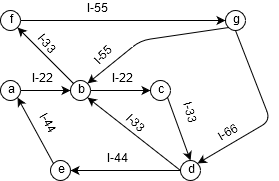
\includegraphics[scale=1]{photos/11-1-27.png} 
				\end{center}
			\item There are two paths from $g$ to $a$. They are:
				\begin{align*}
					& \bm{\{g,d\}, \{d,e\}, \{e,a\}} \textbf{ and}\\ 
					& \bm{\{g,b\},\{b,c\}, \{c,d\}, \{d,e\}, \{e,a\}}
				\end{align*}
			\item In this case it would have to be have to be 2, as there are 2 possible ways to reach $d$ from $b$ so if you shut down roads: \{$g$,$d$\} and \{$c$,$d$\} you make it impossible for $b$ to ever reach $d$
			\item It is impossible as you will hit either towns $b$ or $d$ at least twice. 
			\item If it was an x-y walk then yes, it is absolutely possible. This can be ending at town $g$. This would look like: 
				\begin{align*}
					\bm{\{c,d\}, \{d,e\}, \{e,a\}, \{a,b\}, \{b,f\}, \{f,g\}}
				\end{align*}
			\item Yes it is possible! A simple path that lets you visit at least each of the highways once is:
				\begin{align*}
					\bm{\{e,a\},\{a,b\}, \{b,f\}, \{f,g\},\{g,d\}}
				\end{align*}
		\end{enumerate}
	\end{homeworkProblem} 

	%%%%%%%%%%%%%%%%%%%      
	%	NEW SECTION   %
	%%%%%%%%%%%%%%%%%%%
	\section{Chapter 11.2}
	
	%%%%%%%%%%%%%%%%%%%%%%%%%%%%%%%%%%%%%%%%%%%%%%%%%%%%%%%%%%%%%%%%%%%%%%%%%%%%%%%%%%
	%                                                                                %
	%                          Section 11.2 Problem 1                                %
	%                                                                                %
	%%%%%%%%%%%%%%%%%%%%%%%%%%%%%%%%%%%%%%%%%%%%%%%%%%%%%%%%%%%%%%%%%%%%%%%%%%%%%%%%%%
	
	\begin{homeworkProblem}[Problem 1]
		\tab Let $G$ be the undirected graph in Fig. 11.27(a).
		\begin{enumerate}[label=(\alph*)]
			\item How many connected subgraphs of $G$ have four vertices and include a cycle?
			\item Describe the graph of $G_1$ (of $G$) in part (b) of the figure first, as an induced subgraph and second, in terms of deleting a vertex of $G$.
			\item Describe the graph of $G_2$ (of $G$) in part (c) of the figure first, as an induced subgraph and second, in terms of deleting a vertex of $G$.
			\item Draw the subgraph of $G$ induced by the set of vertices $U$ =\{$b$, $c$, $d$, $f$, $i$, $j$\}.
			\item For the graph $G$, let the edge $e$ = \{$c$, $f$\}. Draw the subgraph $G$ — $e$.
		\end{enumerate}
		
		\begin{center}
			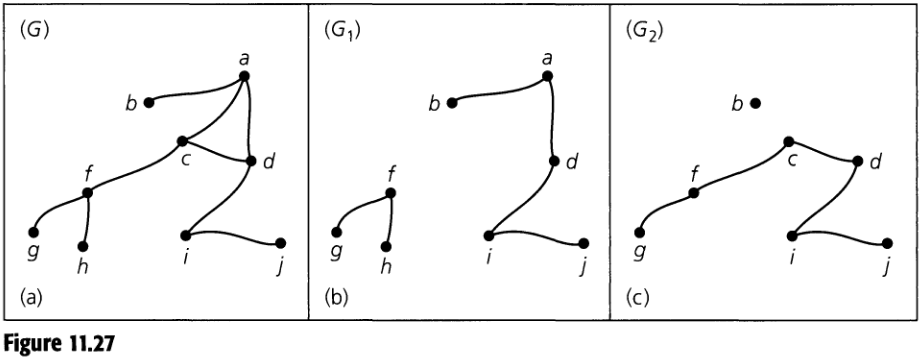
\includegraphics[scale=.67]{photos/1127.png}
		\end{center}
		
		
		\textbf{\\Solution:}
		
		\begin{enumerate}[label=(\alph*)]
			\item There are 3 possible subgraphs of $G$ that have four vertices and include a cycle. They are:
				\begin{align*}
					&\bm{\{b,a\}, \{a,d\}, \{d,c\}, \{c,a\}} \\
					&\bm{\{f,c\}, \{c,d\}, \{d,a\}, \{a,c\}} \\
					&\bm{\{i,d\}, \{d,c\}, \{c,a\}, \{a,d\}}
				\end{align*}
			\item Initially we can say that $G_1$ is induced by the subgraph $U_1=\{a,b,d,f,g,h,i\}$.To describe seondly, in terms of deleting a vertex in $G$ what happened is the vertex $c$ was completely removed from $G$ and all the paths linking to $c$ were also removed.
			\item Initially we can say that $G_2$ is induced by the subgraph $U_2=\{b,c,d,f,g,i\}$.To describe seondly, in terms of deleting a vertex in $G$ what happened is the vertex $a$ and $h$ was completely removed from $G$ and all the paths linking to $a$ and $h$ were also removed.
			\item Here is what that Graph would look like:
				\begin{center}
					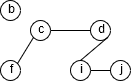
\includegraphics[scale=1]{photos/11-2-1.png}
				\end{center}
			\item In this case we are deleting a line, so the graph would look like:
				\begin{center}
					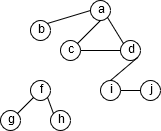
\includegraphics[scale=1]{photos/11-2-1-e.png}
				\end{center}
		\end{enumerate}
		
	\end{homeworkProblem} 

		
	%%%%%%%%%%%%%%%%%%%%%%%%%%%%%%%%%%%%%%%%%%%%%%%%%%%%%%%%%%%%%%%%%%%%%%%%%%%%%%%%%%
	%                                                                                %
	%                          Section 11.2 Problem 3                                %
	%                                                                                %
	%%%%%%%%%%%%%%%%%%%%%%%%%%%%%%%%%%%%%%%%%%%%%%%%%%%%%%%%%%%%%%%%%%%%%%%%%%%%%%%%%%
	
	\begin{homeworkProblem}[Problem 3]
		\begin{enumerate}[label=(\alph*)]
			\item How many spanning subgraphs are there for the graph $G$ in Fig. 11.27(a)?
			\item How many connected spanning subgraphs are there in part (a)?
			\item How many of the spanning subgraphs in part (a) have vertex $a$ as an isolated vertex?
		\end{enumerate}
		
		\textbf{\\Solution:}
		
		\begin{enumerate}[label=(\alph*)]
			\item There are a total of 9 points. This means that there are:
				\begin{align*}
					\bf{2^9}
				\end{align*}
			\item For connected spanning graphs we have to include all cases where the graphs still has all points connected in some sort of way, this is possible in \textbf{4} different ways, as we can exclude a single line from the \{$a$,$b$\}, \{$b$,$c$\}, \{$c$,$a$\} circuit, and still have a connected graph, and then include the original full graph. 
			\item To be isolated we have to remove all the possible paths to $a$, which means that we have to remove the 3 specific edges to $a$. By removing these 3 edges we get:
				\begin{align*}
					\bf{2^6}
				\end{align*}
		\end{enumerate}
		
	\end{homeworkProblem} 

		
	%%%%%%%%%%%%%%%%%%%%%%%%%%%%%%%%%%%%%%%%%%%%%%%%%%%%%%%%%%%%%%%%%%%%%%%%%%%%%%%%%%
	%                                                                                %
	%                          Section 11.2 Problem 9                                %
	%                                                                                %
	%%%%%%%%%%%%%%%%%%%%%%%%%%%%%%%%%%%%%%%%%%%%%%%%%%%%%%%%%%%%%%%%%%%%%%%%%%%%%%%%%%
	
	\begin{homeworkProblem}[Problem 9]
		\tab For each pair of graphs in Fig. 11.29, determine whether or not the graphs are isomorphic.
		\begin{center}
			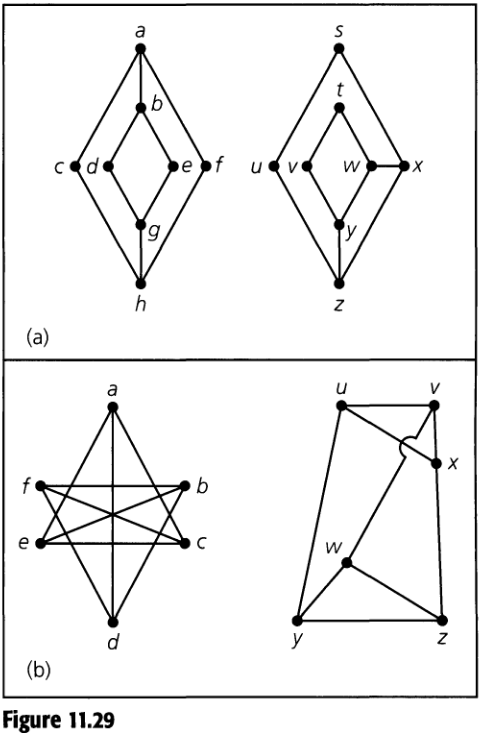
\includegraphics[scale=.5]{photos/1129.png}
		\end{center}
		
		\textbf{\\Solution:}
		\begin{enumerate}[label=(\alph*)]
			\item For this pair it is impossible because the inner points of $b,d,e,g$ and $t,v,w,y$ are impossible to link to each other. This is because $w$ cannot directly connect to $v$ directly. Therefore it is \textbf{not isomorphic}.
			\item This can be done by trying to map each point from the first graph of (b) to the second graph in (b). If we say that $a=w$, $b=u$, $c=z$, $d=v$, $e=y$, $f=x$, we can see that the graphs are able to maintain the same exact relationship with each point. It also has the same amount of vertices and edges so these graphs are \textbf{absolutely isomorphic}.
		\end{enumerate}
		
		
	\end{homeworkProblem} 

		
	%%%%%%%%%%%%%%%%%%%%%%%%%%%%%%%%%%%%%%%%%%%%%%%%%%%%%%%%%%%%%%%%%%%%%%%%%%%%%%%%%%
	%                                                                                %
	%                          Section 11.2 Problem 14                               %
	%                                                                                %
	%%%%%%%%%%%%%%%%%%%%%%%%%%%%%%%%%%%%%%%%%%%%%%%%%%%%%%%%%%%%%%%%%%%%%%%%%%%%%%%%%%
	
	\begin{homeworkProblem}[Problem 14]
		\begin{enumerate}[label=(\alph*)]
			\item Find a graph $G$ where both $G$ and $\bar{G}$ are connected.
			\item If $G$ is a graph on $n$ vertices, for $n\ge{2}$, and $G$ is not
			connected, prove that $\bar{G}$ is connected.
		\end{enumerate} 
		
		
		\textbf{\\Solution:}
		
		\begin{enumerate}[label=(\alph*)]
			\item A simple example is a 4 vertex shape that looks like:
			\begin{center}
				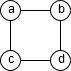
\includegraphics[scale=1]{photos/11-2-14-a-1.png}
			\end{center}
			With its complement looking like:
			\begin{center}
				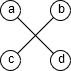
\includegraphics[scale=1]{photos/11-2-14-a-2.png}
			\end{center}
			\item To start, we are looking to see if the complement of a disconnected graph is connected for any $n$ vertices that is greater than 2. So, to keep going, let's say we have a graph of size 4, similar to problem (a) (I think a bigger square will provide better visualization.) The largest incomplete graph I can make will include 3 points, lets say we have the edges \{$a$,$b$\}, \{$b$,$d$\}, \{$a$,$d$\}. This is all the possible lines we can make that do not connect to $c$. Now, in the complement every point will connect to C, creating a connected graph. This is because the complement will include every point connecting to the final point, and this also holds true if you create multiple sub-connected graphs in a larger graph, the points that are not connecting to the "outsider" points will connect in the complement, thus making the complement always connected if the original graph is not. 
		\end{enumerate}
		
		
	\end{homeworkProblem} 

	%%%%%%%%%%%%%%%%%%%      
	%	NEW SECTION   %
	%%%%%%%%%%%%%%%%%%%
	\section{Chapter 11.3}
	
	%%%%%%%%%%%%%%%%%%%%%%%%%%%%%%%%%%%%%%%%%%%%%%%%%%%%%%%%%%%%%%%%%%%%%%%%%%%%%%%%%%
	%                                                                                %
	%                          Section 11.3 Problem 5                                %
	%                                                                                %
	%%%%%%%%%%%%%%%%%%%%%%%%%%%%%%%%%%%%%%%%%%%%%%%%%%%%%%%%%%%%%%%%%%%%%%%%%%%%%%%%%%
	
	\begin{homeworkProblem}[Problem 5]
		\begin{center}
			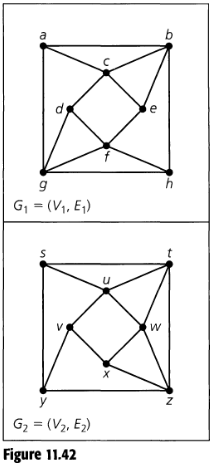
\includegraphics[scale=.7]{photos/fig11-42.png}
		\end{center}
		\tab Let $G_1$ = ($V_1$, $E_1$) and $G_2$ = ($V_2$, $E_2$) be the loop-free undirected connected graphs in Fig. 11.42.
		\begin{enumerate}[label=(\alph*)]
			\item Determine $|V_1|,|E_1|,|V_2|,|E_2|$.
			\item Find the degree of each vertex in $V_1$. Do likewise for each vertex in $V_2$.
			\item Are the graphs $G_1$ and $G_2$ isomorphic
		\end{enumerate}
		
		
		\textbf{\\Solution:}
		
		\begin{enumerate}[label=(\alph*)]
			\item $|V_1|$ = 8, $|E_1|$=14. $|V_2|$ = 8, $|E_2|$=14
			\item so, starting with $|V_1|$ we have:
				\begin{align*}
					a=3,b=4,c=4,d=3,e=3,f=4,g=4,h=3
				\end{align*}
				for $|V_2|$ it is:
				\begin{align*}
					s=3,t=4,u=4,v=3,w=4,x=3,y=3,z=4
				\end{align*}
				both $|V_1|$ and $|V_2|$ have 4 vertices of degree 3, and 4 vertices of degree 4. 
			\item $G_1$ and $G_2$ are not isomorphic, and we can see why in the inner square of points. We can see that the vertices $d$, and $x$, have 3 possible partners, and are centered, However in $G_1$ we can see that $c$ connects to only points with degree 4, whereas $x$ will connect to a point $v$ with degree 3. The relationships between each vertice is impossible to maintain, therefore they are not isomorphic.  
		\end{enumerate}
		
		
	\end{homeworkProblem} 

	%%%%%%%%%%%%%%%%%%%%%%%%%%%%%%%%%%%%%%%%%%%%%%%%%%%%%%%%%%%%%%%%%%%%%%%%%%%%%%%%%%
	%                                                                                %
	%                          Section 11.3 Problem 8                                %
	%                                                                                %
	%%%%%%%%%%%%%%%%%%%%%%%%%%%%%%%%%%%%%%%%%%%%%%%%%%%%%%%%%%%%%%%%%%%%%%%%%%%%%%%%%%
	
	\begin{homeworkProblem}[Problem 8]
		\begin{enumerate}[label=(\alph*)]
			\item Find the number of edges in $Q_8$
			\item Find the maximum distance between pairs of vertices in $Q_8$. Give an example of one such pair that achieves this distance.
			\item Find the length of a longest path in $Q_8$
		\end{enumerate}
		
		
		\textbf{\\Solution:}
		
		\begin{enumerate}[label=(\alph*)]
			\item The number of edges is equal to the equation:
				\begin{align*}
					2^{n-1}\times n
				\end{align*}
				\tab in this case $n=8$. As a result, you would end up with an equation that looks like:
				\begin{align*}
					2^7\times 8=\bf{1,024}
				\end{align*}
			\item The maximum distance between a pair of vertices in $Q_8$ would be the $n^{\text{th}}$ dimension of the cube, thus being 8. We can find the furthest most point by flipping each bit value in the vertice. For example: if we had values 01010101, the furthest point in the hypercube from this is 1010101. This is because each bit is a single dimension being changed, so by flipping the bit you are on the other side of that dimension (This can be easier imagined with a 3 dimensional cube following the x,y,z axis. If 000 is the top left corner closest to you the value 111 would be the bottom right corner furthest from you). Therefore, the answer in this case is \textbf{8}
			\item A path is the furthest you can travel without repeating a vertex. In this case, the furthest that you could travel without repeating vertices. You could, theoretically hit every point before returning back to the original point. Of course because you can't traverse each point because a repeating vertex means it is not a path. So we can hit every point, without repeats, meaning that you can hit:
				\begin{align*}
					\bf{2^8-1=255}
				\end{align*}
		\end{enumerate}
		
	\end{homeworkProblem} 

	%%%%%%%%%%%%%%%%%%%%%%%%%%%%%%%%%%%%%%%%%%%%%%%%%%%%%%%%%%%%%%%%%%%%%%%%%%%%%%%%%%
	%                                                                                %
	%                          Section 11.3 Problem 30                               %
	%                                                                                %
	%%%%%%%%%%%%%%%%%%%%%%%%%%%%%%%%%%%%%%%%%%%%%%%%%%%%%%%%%%%%%%%%%%%%%%%%%%%%%%%%%%
	
	\begin{homeworkProblem}[Problem 30]
		\tab Carolyn and Richard attended a party with three other married couples. At this party a good deal of handshaking took place, but
		\begin{enumerate}[label=(\arabic*)]
			\item no one shook hands with her or his spouse;
			\item no one shook hands with herself or himself; and 
			\item no one shook hands with anyone more than once.
		\end{enumerate}
		\tab Before leaving the party, Carolyn asked the other seven people how many hands she or he had shaken. She received a different answer from each of the seven. How many times did Carolyn shake hands at this party? How many times did Richard?
		
		\textbf{\\Solution:\\}
		\tab To start we can get a part of the answer from the hints. No person shook hands with themselves, or their spouse, which means that of the 8 people a person can shake hands with, at most, 6 people, and at fewest 0. This means that there were 7 possible answers that would fit the criteria. If there were 7 different responses at the end of the night that means that Carolyn has to be one of the values that was repeated, as there were 8 people and only 7 possible amounts of hands to shake following the rules it means Carolyn is one of the repeat values. Now, from here we can try and determine who shook who's hand.
		
		\tab Now, let's start by creating a graph with a bunch of couples. Let's say some person shakes hands with 6 people. This would look like:
		\begin{center}
			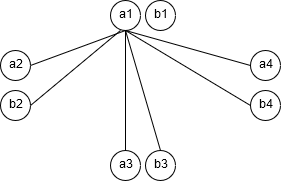
\includegraphics[scale=.5]{photos/11-3-30-1.png}
		\end{center}
	
		\tab In this graph the letter indicates a specific person in a couple, and the number indicates whether the couples belong to each other. So person $a$ in couple $1$ is paired with person $b$ in couple $2$. What I did here is connect a person to 6 other people, following the rules. Now, because I there is only 1 person, $a1$'s spouse, $b1$ who has 0 connected to it, it can be assumed that they will hold 0. In the next graph we will go to couple 2 and make one of the couples link to 5 people. This would look like:
		\begin{center}
			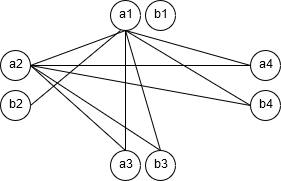
\includegraphics[scale=.5]{photos/11-3-30-2.png}
		\end{center}
		
		\tab Now, what we see here is that we connected $a2$ to every possible option it could connect to that was not $b1$ in order to maintain that as a 0 point. What this did is it made $a2$ have 5 and left $b2$ as the only option left to complete 1 handshake. This couple, now, is also complete, and we can not change their values. Let us now go to $a3$ and see if we can make it 4 while still maintaining the first and second couples numbers. This would look like:
		\begin{center}
			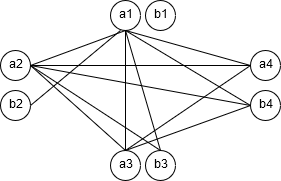
\includegraphics[scale=.5]{photos/11-3-30-3.png}
		\end{center}
	
		\tab This ends up being the final graph, as we have all 6 values reached and notice that 3 is the repeating value. Now, we know that 3 is the repeating value we know that this occurs at the vertice $a4$, so we can say that this point is Caroline. Her partner, Richard, is in couple 4 with Caroline, and also has a value of 3. Therefore, \textbf{Both Caroline and Richard each shook 3 hands}
	
	\end{homeworkProblem} 

	%%%%%%%%%%%%%%%%%%%      
	%	NEW SECTION   %
	%%%%%%%%%%%%%%%%%%%
	\section{Chapter 11.4}
	
	%%%%%%%%%%%%%%%%%%%%%%%%%%%%%%%%%%%%%%%%%%%%%%%%%%%%%%%%%%%%%%%%%%%%%%%%%%%%%%%%%%
	%                                                                                %
	%                          Section 11.4 Problem 5                                %
	%                                                                                %
	%%%%%%%%%%%%%%%%%%%%%%%%%%%%%%%%%%%%%%%%%%%%%%%%%%%%%%%%%%%%%%%%%%%%%%%%%%%%%%%%%%
	
	\begin{homeworkProblem}[Problem 5]
		\tab For each graph in Fig. 11.68 determine whether or not the graph is bipartite.
		\begin{center}
			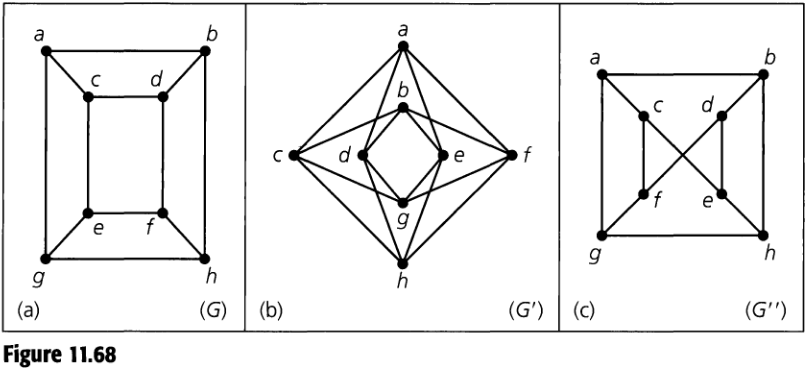
\includegraphics[scale=.6]{photos/1168.png}
		\end{center}
		\textbf{\\Solution:}
		\begin{enumerate}[label=(\alph*)]
			\item Yes, this graph is bipartite because we can write $V_1$ and $V_2$, very similarly to graph represented in the book at figure 11.49, $V_1=\{e,a,h,d\}$ and $V_2=\{b,c,f,g\}$. Every point in $G$ is in $V_1 \cup V_2$, and every point in $V_1 \cap V_2 = \emptyset$.
			\item This graph is also bipartite because we can write $V_1 = \{c,d,e,f\}$ and $V_2 = \{a,b,g,h\}$. Every point in $G$ is in $V_1 \cup V_2$, and every point in $V_1 \cap V_2 = \emptyset$.
			\item This last graph is not bipartite because there is no way to separate the graph into two groups where the points are not connecting in each group, they don't have any way to connect without some intersection between the two groups, so it is impossible to make a bipartite graph. 
		\end{enumerate}
		
		
	\end{homeworkProblem} 

	%%%%%%%%%%%%%%%%%%%%%%%%%%%%%%%%%%%%%%%%%%%%%%%%%%%%%%%%%%%%%%%%%%%%%%%%%%%%%%%%%%
	%                                                                                %
	%                          Section 11.4 Problem 9                                %
	%                                                                                %
	%%%%%%%%%%%%%%%%%%%%%%%%%%%%%%%%%%%%%%%%%%%%%%%%%%%%%%%%%%%%%%%%%%%%%%%%%%%%%%%%%%
	
	\begin{homeworkProblem}[Problem 9]
		\tab How many paths of longest length are there in each of the following graphs? (Remember that a path such as $v_1 \rightarrow v_2 \rightarrow v_3$ is considered to be the same as the path $v_3 \rightarrow v_2 \rightarrow v_3.$)
		\begin{enumerate}[label=(\alph*)]
			\item $K_{1,4}$ 
			\item $K_{3,7}$
			\item $K_{7,12}$
			\item $K_{m,n}$, where $m,n\in \mathbb{Z}^+$ with $m<n$.
		\end{enumerate}
		
		\textbf{\\Solution:}
		
		\begin{enumerate}[label=(\alph*)]
			\item $\frac{1}{2}(4)(1)(3)=6$
			\item $\frac{1}{2}(7)(3)(6)(2)(5)(1)(4)=2,520$
			\item $\frac{1}{2}(12)(7)(11)(6)(10)(5)(9)(4)(8)(3)(7)(2)(6)(1)(5)=50,295,168,000$
			\item $\frac{1}{2}(n)(m)(n-1)(m-1)...(2)(n-(m+1))(1)(n-m)$
		\end{enumerate}
		
	\end{homeworkProblem} 

	%%%%%%%%%%%%%%%%%%%%%%%%%%%%%%%%%%%%%%%%%%%%%%%%%%%%%%%%%%%%%%%%%%%%%%%%%%%%%%%%%%
	%                                                                                %
	%                          Section 11.4 Problem 17                               %
	%                                                                                %
	%%%%%%%%%%%%%%%%%%%%%%%%%%%%%%%%%%%%%%%%%%%%%%%%%%%%%%%%%%%%%%%%%%%%%%%%%%%%%%%%%%
	
	\begin{homeworkProblem}[Problem 17]
		\tab Determine the number of vertices, the number of edges, and the number of regions for each of the planar graphs in Fig. 11.71. Then show that your answers satisfy Euler's Theorem for connected planar graphs.
		\begin{center}
			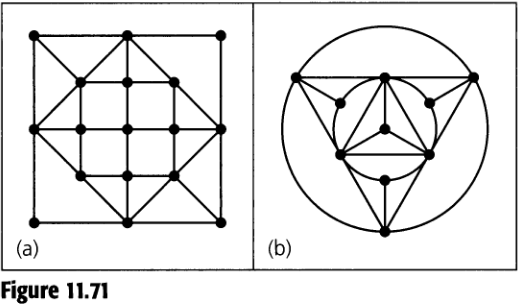
\includegraphics[scale=.7]{photos/1171.png}
		\end{center}
		
		\textbf{\\Solution:}
		
		\begin{enumerate}[label=(\alph*)]
			\item figure (a) has a total of 17 vertices and 34 edges. Counting the regions in this graph, there are a total of 19. To follow the theorom, we do vertices-edge+regions. This looks like:
				\begin{align*}
					\bf{17-34+19=2}
				\end{align*}
			\item figure (b) has a total of 10 vertices and 24 edges. Counting the regions in this graph, there are a total of 16. To follow the theorom:
				\begin{align*}
					\bf{10-24+16=2}
				\end{align*}
		\end{enumerate}

		
	\end{homeworkProblem} 

	%%%%%%%%%%%%%%%%%%%      
	%	NEW SECTION   %
	%%%%%%%%%%%%%%%%%%%
	\section{Chapter 11.5}
	
	%%%%%%%%%%%%%%%%%%%%%%%%%%%%%%%%%%%%%%%%%%%%%%%%%%%%%%%%%%%%%%%%%%%%%%%%%%%%%%%%%%
	%                                                                                %
	%                          Section 11.5 Problem 1                                %
	%                                                                                %
	%%%%%%%%%%%%%%%%%%%%%%%%%%%%%%%%%%%%%%%%%%%%%%%%%%%%%%%%%%%%%%%%%%%%%%%%%%%%%%%%%%
	
	\begin{homeworkProblem}[Problem 1]
		\tab Give an example of a connected graph that has
		\begin{enumerate}[label=(\alph*)]
			\item Neither an Euler circuit nor a Hamilton cycle,
			\item An Euler circuit but no Hamilton cycle.
			\item A Hamilton cycle but no Euler circuit
			\item Both a Hamilton cycle and an Euler circuit
		\end{enumerate}
		
		\textbf{\\Solution:}
		
		\begin{enumerate}[label=(\alph*)]
			\item An example of neither an Euler circuit nor a Hamilton cycle would look like:
				\begin{center}
					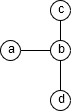
\includegraphics[scale=1]{photos/11-5-1-a.png}
				\end{center}
				In this example it is impossible to create an euler circuit as you have to cross at least one edge twice in order to get to another edge, and it is an impossible Hamilton cycle because you have to repeat vertex $b$ at least more than once to reach each vertex.
			\item An example of an Euler Circuit but not a Hamilton cycle is:
				\begin{center}
					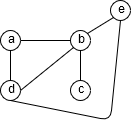
\includegraphics[scale=1]{photos/11-5-1-b.png}
				\end{center}
				This is an example of a Euler circuit as if you follow the trail: $c-b-a-d-e-b-d$. This ends up being an Euler circuit as I visit every possible edge only once before returning, but, in the process, end up visiting the vertice b twice.
			\item An example of a graph with a Hamilton cycle but no Euler circuit is:
				\begin{center}
					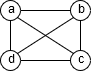
\includegraphics[scale=1]{photos/11-5-1-c.png}
				\end{center}
				\tab Here we can traverse the graph and get a Hamilton cycle by following the path: $a-b-c-d$. However, it is impossible to create an Euler cycle because you have to repeat at least one edge more than once. In this way it is a Hamilton cycle and not an Euler circuit.
			\item An example of both a Hamilton Cycle and an Euler circuit is this graph:
				\begin{center}
					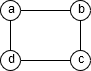
\includegraphics[scale=1]{photos/11-5-1-d.png}
				\end{center}
				\tab Starting at any point it is possible traverse around the square, and land back at the original point started. In the process you will visit every possible edge and vertice, making it both a Hamilton cycle and an Euler Circuit.
		\end{enumerate}
		
	\end{homeworkProblem} 

	%%%%%%%%%%%%%%%%%%%%%%%%%%%%%%%%%%%%%%%%%%%%%%%%%%%%%%%%%%%%%%%%%%%%%%%%%%%%%%%%%%
	%                                                                                %
	%                          Section 11.5 Problem 3                                %
	%                                                                                %
	%%%%%%%%%%%%%%%%%%%%%%%%%%%%%%%%%%%%%%%%%%%%%%%%%%%%%%%%%%%%%%%%%%%%%%%%%%%%%%%%%%
	
	\begin{homeworkProblem}[Problem 3]
		\tab Find a Hamilton cycle, if one exists, for each of the graphs or multigraphs in Fig. 11.84. If the graph has no Hamilton cycle, determine whether it has a Hamilton path. 
		\begin{center}
			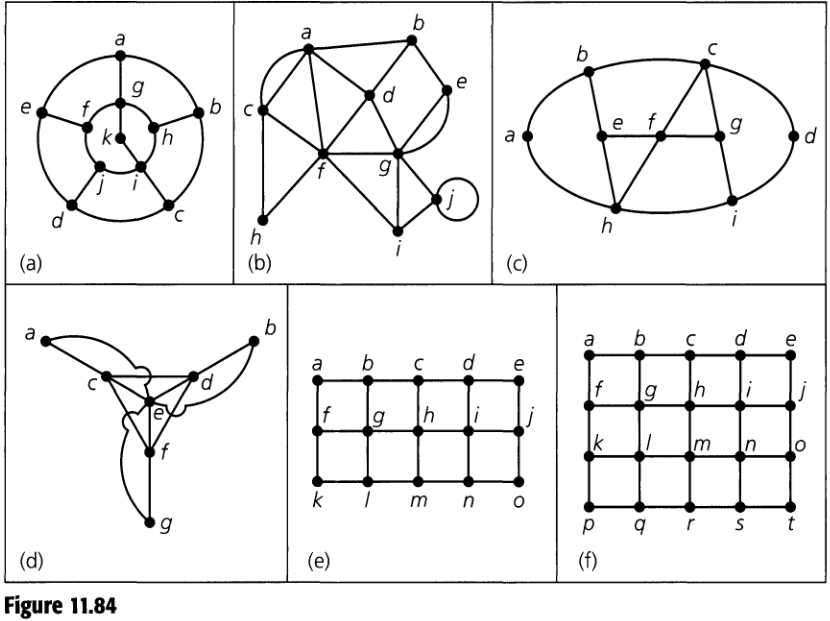
\includegraphics[scale=.5]{photos/1184.png}
		\end{center}
		\textbf{\\Solution:}
		\begin{enumerate}[label=(\alph*)]
			\item For graph (a) It is a Hamilton cycle, the Hamilton cycle follows the path: $k-i-h-b-c-d-j-f-e-a-g-k$. You can do this by starting at $c$ then follow the trail $d-e-a-b-h-g-f-j-i-k$. 
			\item Graph (b) also has a Hamilton cycle, as it follows the path: $f-h-c-a-d-b-e-g-j-i-f$. You can also make a Hamilton path by: $f-h-c-a-d-b-e-g-j-i$
			\item Graph (c) also has a Hamilton cycle. You can get this by: $a-b-c-d-i-g-f-e-h-a$. You can get a Hamilton path by: $a-b-c-d-i-g-f-e-h$
			\item Graph (d) does not have a Hamilton cycle. It does, however, have a Hamilton path, the Hamilton path would look like: $b-d-f-g-e-a-c$
			\item Graph (e) does not have a Hamilton cycle, but it does have a Hamilton path. The Hamilton path would look like: $a-b-c-d-e-j-i-h-g-f-k-l-m-n-o$
			\item Graph (f) does have a Hamilton cycle, this cycle could look like: $b-a-f-k-p-q-l-m-r-s-t-o-n-i-j-e-d-c-h-g-b$. A Hamilton path could similarly look like: $b-a-f-k-p-q-l-m-r-s-t-o-n-i-j-e-d-c-h-g$
		\end{enumerate}
		
		
	\end{homeworkProblem} 

	%%%%%%%%%%%%%%%%%%%%%%%%%%%%%%%%%%%%%%%%%%%%%%%%%%%%%%%%%%%%%%%%%%%%%%%%%%%%%%%%%%
	%                                                                                %
	%                          Section 11.5 Problem 12                               %
	%                                                                                %
	%%%%%%%%%%%%%%%%%%%%%%%%%%%%%%%%%%%%%%%%%%%%%%%%%%%%%%%%%%%%%%%%%%%%%%%%%%%%%%%%%%
	
	\begin{homeworkProblem}[Problem 12]
		\tab Prove that for $n\ge{2}$, the hypercube $Q_n$ has a Hamilton cycle.
		
		\textbf{\\Solution:\\}
		\tab I believe this can be solved inductively. To start, lets check a base case, starting with a hypercube $Q_2$. This is basically a square, it would look like:
		\begin{center}
			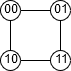
\includegraphics[scale=1]{photos/11-5-12-1.png}
		\end{center}
	
		\tab This absolutely has a Hamilton cycle, so this basis case is proven correct. After this we can try to see if we can solve it inductively based on assuming that $Q_n$ has a Hamilton cycle. Let's see what will happen with $Q_{n+1}$. We know, for example, that $Q_{n+1}$ is 2 connected $Q_n$, like how $Q_3$ is a cube which is 2 connected $Q_2$ squares. We know that $Q_n$ has a Hamilton cycle, so we know each piece, before being put together, has a Hamilton cycle. Now, in its connection there are an even number of connections that form a cycle of some sort, allowing you to start back in the position you began from, therefore allowing you to create a Hamilton cycle. 
		
		
	\end{homeworkProblem} 
\end{document}